\section{Problemstellung}
\label{problemstellung}

Diese Arbeit beschäftigt


% , die dessen Konzepte auf Graphen ü

% Einführen und Arbeit zusammenfassen.

% Wir zeigen, dass wir bisherige Faltungsoperatoren auf Graphen drastisch verbessern können, wenn den Graphenkanten eine Orientierung zu Grunde liegt und wir diese berücksichtigen.

% Wir zeigen, dass die Vorgestellten Faltungsoperatoren in dieser Arbeit äquivalent zu der Köassischen Faltung auf rwgulären Gittern aind und
% Obwohl diese nicht ganz mit den klassischen Faltungsoperatoren auf Bildern für irreguläre Graphen mithalten könn n, so zeigen sie sich dennoch als lohnenswert auf Grundlage ihrer Datenreduktion für zukünftige Arbeiten.
% gerade in Hinsicht für eine effiziente GPU Implementierung.

% CNNs falten selbst die unnötigsten Stellen eines Bildes, wohingegen der Graphansatz durch eine Vorverarbeitung diesw zu einem Knoten zusammenfügt.

% Insbesondere hier schon auf räumlich und spektral eingehen, da es woanders keinen sinn macht

% In the context of the generalization of Convolutional Neural Networks (CNNs) to irregular domains modelled by graphs, the problem is the classification or regression of graph signals, i.e.\ signals who take a value at each vertex of a weighted graph. There is two approaches to convolve a graph signal with a (learned) filter:
% Spatially sliding a filter on the vertices, as you would slide a filter on a 2D image or a 1D audio signal (the pixels form a grid graph, the time forms a line graph), i.e.\ the straightforward application of the definition of a convolution. This approach however presents two challenges: (1) the definition of a receptive field / neighbourhood, because sampling on arbitrary graphs is not necessarily uniform and (2), the ordering of nodes, because problem-specific ordering, e.g.\ spatially ordered pixels or time ordered samples, is missing. These recent works, who present the same ideas differently, spatially define the convolution operator on graphs:
% The spectral formulation builds on Spectral Graph Theory and Computational Harmonic Analysis. It decomposes the graph Laplacian (via an eigendecomposition) to form a Fourier basis, which properties are analog to the classical Fourier basis on n-dimensional Euclidean spaces. A convolution in the graph domain is then equivalent to a multiplication in the spectral domain. See [1211.0053] for an overview of the Graph Signal Processing field. Note that the spectral approach was also proposed in [1312.5851] (using FFTs) to speed up CNNs on regular 2D Euclidean spaces (i.e.\ for images). The limitations of this approach is (for now, we have plans to address those): (1) filters are rotation invariant, and (2) filters are not directly transferrable to a different graph. These recent works, who build on one another, spectrally define the convolution operator on graphs:

% Generell Lernen auf Graphen, die in der Ebene oder im Raum eingebettet sind, z.B. Straßennetze, Karten.


\begin{figure}[t]
\centering
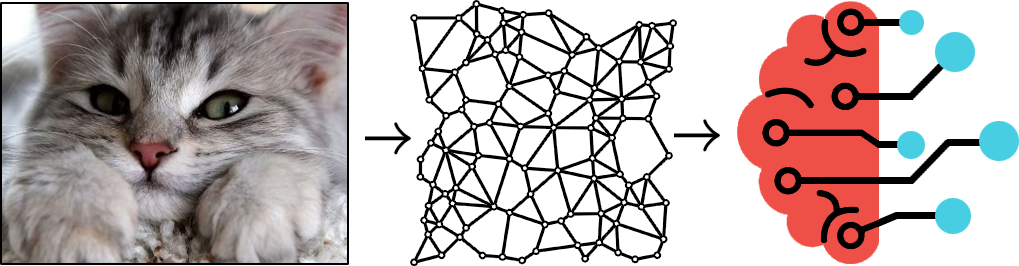
\includegraphics[width=0.9\textwidth]{bilder/problemstellung.png}
\caption[Problemstellung]{Bilder werden in dieser Arbeit für ihre Eingabe in ein neuronales Netz zuvor in eine korrespondierende Graphrepräsentationen konvertiert\protect\footnotemark.}
\label{fig:problemstellung}
\end{figure}
\footnotetext{\url{https://www.shutterstock.com/g/ArtRoseStudio}}

